%\documentclass[iop]{emulateapj-rtx4}
% \shortauthors{French $\&$ Wakker}
%
%\usepackage{graphicx}
%\usepackage{subfigure}
%\usepackage{hyperref}
%\usepackage{amsmath}


%%%%%%%%%%
\documentclass[twocolumn,tighten]{aastex62}
%\documentclass{aastex6}
%\usepackage{emulateapj-rtx4}
%\usepackage{emulateapj}

 \shortauthors{French $\&$ Wakker}
\usepackage{graphicx}
\usepackage{subfigure}
\usepackage{amsmath}

%\usepackage{dblfloatfix}

%\usepackage{longtable}
%\usepackage{deluxetable}


\newcommand{\kms}{$\rm km\, s^{-1}$}
\newcommand{\HI}{\mbox{H\,{\sc i}} }

%\newcommand{\HI}{H\,{\sc i}}


\newcommand{\I}{\,{\sc i}}
\newcommand{\II}{\,{\sc ii}}
\newcommand{\III}{\,{\sc iii}}
\newcommand{\IV}{\,{\sc iv}}
\newcommand{\V}{\,{\sc v}}
\newcommand{\VI}{\,{\sc vi}}


\graphicspath{{figures//}}

\begin{document}

%\title{The environmental dependence of low-$z$ Ly$\alpha$ absorption}
\title{INTRODUCTION}


%Do Ly$\alpha$ absorbers co-rotate with galaxies?}

\author{David M. French}

\affil{Department of Astronomy, University of Wisconsin, Madison, WI 53706, USA}

\begin{abstract}

Galaxies must accrete gas from the intergalactic medium (IGM) in order to sustain star formation at observed levels. In order to understand this complex process, and how it influences galaxy evolution globally, it is necessary to understand the physical conditions and distribution of the gas around galaxies, known as the circumgalactic medium (CGM). This thesis aims to address these questions through the largest-to-date survey of low column density $\rm Ly\alpha$ absorption detected in the spectra of background QSOs taken by the Cosmic Origins Spectrograph (COS) on the Hubble Space Telescope (HST). By correlating the positions of detection absorption lines with the surrounding galaxy environment, I aim to gain insights to the complex relationship between intergalactic gas and the galaxies which feed on it. This introduction provides some historical and astrophysical perspective, as well as an overview of the methods and history of QSO absorption line spectroscopy.

\end{abstract}

\keywords{galaxies:intergalactic medium, galaxies:evolution, galaxies:halos, quasars: absorption lines}


\section{Overview of the Circumgalactic Medium}

The majority of the baryons in the universe are found in the diffuse intergalactic medium (IGM). The IGM and the galaxies that reside in it are tightly linked by processes such as feedback and accretion. In order to sustain the level of star formation observed, galaxies must accrete gas throughout their lifetimes (e.g., \citealt{erb2008, putman2009a, putman2009b, prochaska2009, bauermeister2010, genzel2010}). At the same time, ongoing star formation and active galactic nuclei (AGN) activity produce feedback that drives gas back into the IGM. This life cycle of gas is complex, and difficult to constrain observationally. Understanding the properties of the IGM, such as its densities, temperatures, motions, and its relationship to the galaxies embedded within it is \emph{essential} for explaining the evolution of galaxies and the star formation history of the Universe. 

The properties of the vast reservoir of material in the IGM can be understood by analyzing lines of sight toward background quasi-stellar objects (QSOs). Individual concentrations of gas along a given sightline imprint a `forest' of absorption lines on the spectrum in the direction of the QSO target. The metal lines trace the star formation history within the intervening gas, and neutral hydrogen lines ($\rm Ly\alpha$ is one of the most commonly and easily observed) indicate both the location and velocities of outflowing gas, as well as the presence of fuel for future star formation. Figure \ref{cgm_artist} shows an artists impression of a galaxy complete with a CGM halo with arrows indicating outflowing and recycling material, and an illustration of a HST sightline detecting halo gas absorption. The relationship between the galaxies and the IGM is usually studied by looking for galaxies that lie at similar redshifts as detected absorption lines. This approach has value but is incomplete; it does not allow for an unbiased understanding of the distribution of the gas around galaxies, which requires looking for both detections and non-detections of gas, both near as well as far away from galaxies.

The current standard model of structure formation is given by Lambda Cold-Dark-Matter ($\Lambda$CDM) cosmology, which predicts the hierarchical growth of large scale structures seeded by initial fluctuations in the dark matter background. In this picture, both galaxies and the IGM should follow the same underlying density profile. Some observational evidence of this large-scale relationship has appeared recently, such as \cite{wakker2015}, who showed that $\rm Ly\alpha$ absorption strength (equivalent width; EW) traces the overall distribution of galaxies in a Cosmic Web filament. Figure \ref{wakker_filament} shows their plot of the EW of $\rm Ly\alpha$ absorbers as a function of distance to the center of a galaxy filament, with the enhanced absorption strength evident close to the filament center. In addition, numerous studies have shown that $\rm Ly\alpha$ absorbers also trace individual galaxy halos (e.g., \citealt{wakker2009, danforth2016, stocke2013, liang2014, lanzetta1995, chen1998, chen2001a, tripp1998, steidel2010, prochaska2011, thom2012})


\begin{figure}[ht!]
        \centering
        \vspace{0pt}
        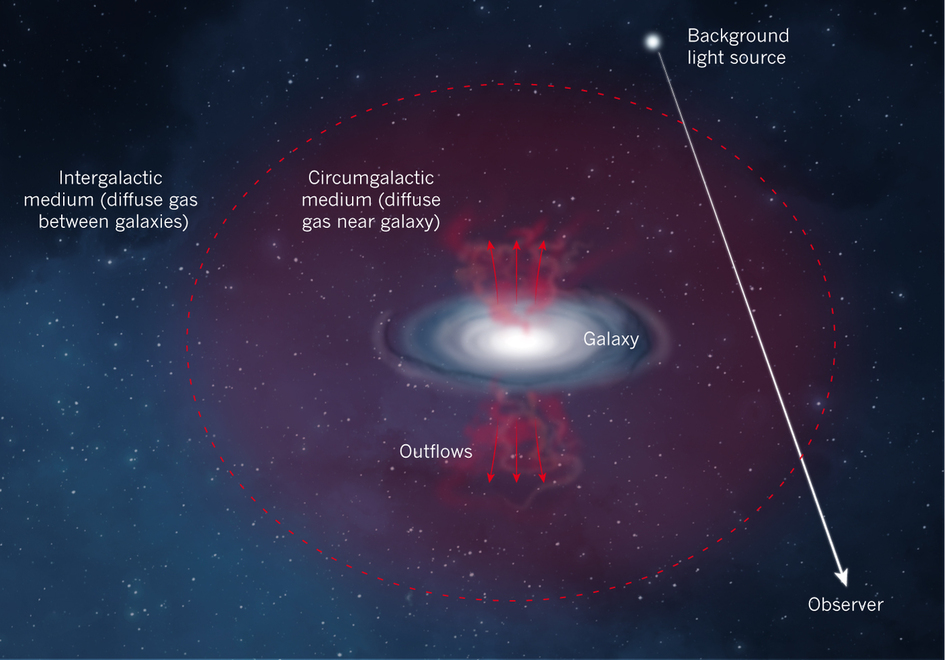
\includegraphics[width=0.49\textwidth]{cgm_nature.jpg}
        \caption{\small{An artist's impression of the CGM of a galaxy. Image credit: NASA/STScI/Ann Feild}}
        \vspace{5pt}
        \label{cgm_artist}
\end{figure}


\begin{figure}[ht!]
        \centering
        \vspace{0pt}
        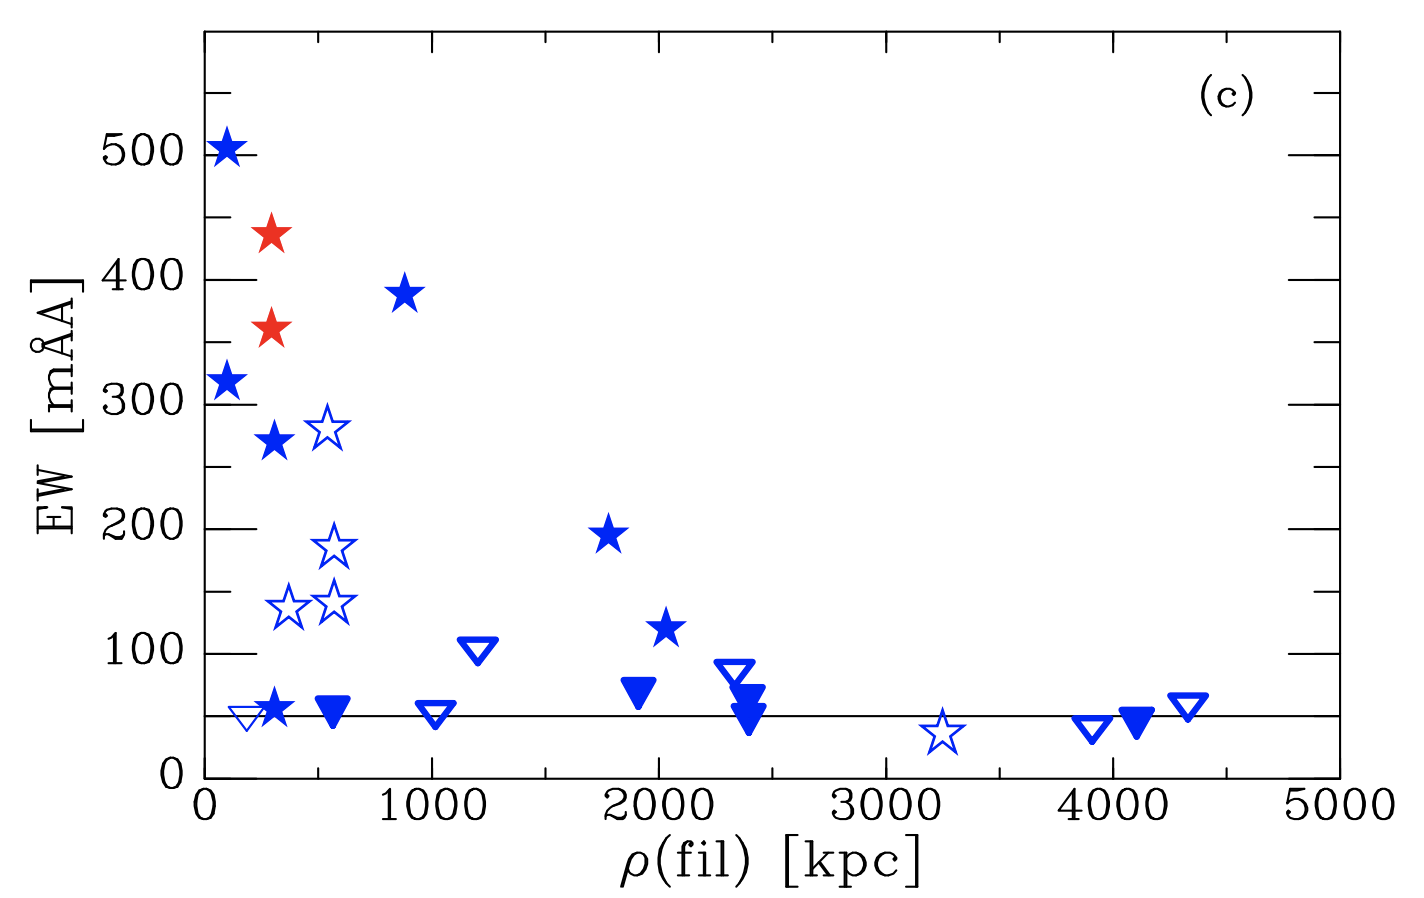
\includegraphics[width=0.49\textwidth]{Wakker2015_filament_EW.png}
        \caption{\small{The EW of $\rm Ly\alpha$ absorbers as a function of distance to the center of a galaxy filament. Blue downward tracing triangles indicate upper limits for non-detection, and all stars indicate detections. See \cite{wakker2015}.}}
        \vspace{5pt}
        \label{wakker_filament}
\end{figure}


Recent studies find that about half of $\rm Ly\alpha$ absorbers lie within galaxy halos, at impact parameters $\rho \lesssim 350$ kpc \citep{cote2005, prochaska2006}. In addition, \cite{wakker2009} find that for 90\% of $L > 0.1 L^{\**}$ galaxies an absorber can be found within 400 kpc and 400 \kms~, and all galaxies have a $\rm Ly\alpha$ absorber within 1.5 Mpc. Higher redshift studies, such as \cite{rudie2012a} at $2 < z < 3$, find evidence for an elevated density of absorbers up to 2 Mpc from galaxies. \cite{wakker2009} also confirmed a previously suggested correlation between $\rm Ly\alpha$ absorption linewidth (also called Doppler $b$-parameter) and impact parameter ($\rho$), observing that the broadest lines (FWHM $>150$ \kms) are only seen within 350 kpc of a galaxy, while only narrower lines (FWHM $<75$ \kms) are found at $\rho > 1$ Mpc (see Figure \ref{wakker2009_linewidth}).

In addition, studying the enrichment of galaxy halos is necessary for constraining outflow models and informing stellar feedback prescriptions. Directly measuring the velocity field and column densities of absorbers as a function of impact parameter and orientation around galaxies would provide the clearest evidence of inflow or outflow activity, but results are few and uncertain. \cite{kacprzak2011_inclination} claim to find that Mg\II~ equivalent widths correlate with galaxy inclination but \cite{mathes2014} find no such correlation for $\rm Ly\alpha$ and O\VI absorbers. Furthermore, we should expect outflowing gas to be more highly enriched and trace the metallicity of the associated galaxy, with inflowing gas instead appearing only in \HI. Both \cite{stocke2013} and \cite{liang2014} find an ``edge" to heavy ion absorption at $\sim 0.5 R_{\rm vir}$, but with $\rm Ly\alpha$ covering fractions of $\sim 0.75 - 1$ continuing out to $R_{\rm vir}$. However, \cite{mathes2014} measure O\VI absorption out to $\sim 3 R_{\rm vir}$.

All these previous studies have suffered from small sample sizes (fewer than 50 systems), and incompleteness due to their higher mean redshifts. 




The CGM is commonly split into a two gas phases: a hot, mostly collisionally ionized phase with gas temperatures near $T\gtrsim 10^6$ K, and a cool, mostly photoionzied phase with gas temperatures near $T \lesssim 10^4$ K.

%\cite{lanzetta1995, bowen1996, chen2008, steidel2010, prochaska2011b, wakker2009}


\subsection{Equivalent Width}

\subsection{Doppler b-parameter}



\subsection{Azimuth}


\section{Science Goals}
Four questions:
1.
2.
3.
4.

\subsection{Galaxy Proximity}


\subsection{Galaxy Orientation}


\subsection{Galaxy Rotation}



\section{Summary of Thesis}
In the following chapters I describe a program to observationally explore the connections between low column density $\rm Ly\alpha$ absorption and the galaxy environment in the local Universe. This program focuses mainly on archival QSO observations taken by the Cosmic Origins Spectrograph (COS) on the Hubble Space Telescope (HST), and correlations between the locations of detected $\rm Ly\alpha$ absorption and of galaxies larger than $\sim 0.1 L^{\**}$. By restricting our study to low-redshifts ($cz \leq 10,000$ \kms) we are able to compile a dataset of unparalleled size while remaining highly complete to galaxies of all types, sizes, and distances from absorption detections. 

The results of this these are presented as follows:

1. In Chapter 1 I present a new nearby galaxy catalog. In order to study the CGM-galaxy connection on a large, all-sky scale, we rely heavily on archival, publicly available data for the positions and properties of the galaxies. We 

 
2. In Chapter 2 I present the results of a pilot study with 33 QSO sightlines chosen for their proximity to large galaxies ($D \ge 25$ kpc). We introduce a new method for absorber-galaxy matching, which will make it possible to algorithmically study our large final data set. 

3. In Chapter 3 I present the results of a study of the kinematic connection between galaxy disks and $\rm Ly\alpha$-traced halo gas. 

4. In Chapter 4 I present the results of our full CGM survey, which includes 1135 $\rm Ly\alpha$ absorbers detected in the spectra of 264 QSO spectra.

5. In Chapter 5 I summarize the results of this thesis, and place these results in the broader context of the circumgalactic medium and it's implications for global galaxy evolution.



%\nocite{*}
%\bibliography{rotation_bib}
%\bibliography{/Users/frenchd/Research/bib}{}
\bibliography{/Users/frenchd/Research/inclination/git_inclination/bib}{}
\bibliographystyle{apj}

\clearpage

\appendix

\end{document}
